\chapter{توازنات حمض--قاعدة وطريقة التفاعل الغالب}\label{ch:b1:predominant-reaction}

يذيب الخل ترسبات الكلس في الغلاية؛ وكذلك يفعل عصير الليمون، أسرع قليلًا.
ويحفظ الدم الرقم الهيدروجيني بين حدين ضيقين مهما أكلنا؛ والمشروب
الغازي حمضي بسبب ثنائي أكسيد الكربون المذاب فيه. وكل
هذه توازنات حمض--قاعدة في الماء، والكيميائي الذي يواجه
محلولًا يحوي عدة أحماض وقواعد --- خليطًا، أو محلولًا منظمًا، أو
حمضًا متعدد البروتونات --- يحتاج إلى طريقة موثوقة لإيجاد pH المحلول
وتراكيز أنواعه. يبني هذا الفصل تلك الطريقة: سلّم
للقوة، ومخططات للغلبة، و\emph{طريقة \omterm{def:b1:predominant-reaction:predominant-reaction}{التفاعل
الغالب}}، التي ترد كل خليط إلى التفاعل الوحيد الذي يهم.

\begin{recall}
عرّف الكتاب الأول (الصف الثاني عشر) أحماض برونستد وقواعده، \omterm{def:b1:predominant-reaction:acidity-constant}{وثابت الحمضية}
$K_a$ و$\mathrm{p}K_a$، \omterm{def:b1:predominant-reaction:autoprotolysis}{والجداء الأيوني للماء} وpH الأحماض
\omterm{def:b1:predominant-reaction:strong-acid}{والقواعد القوية}، ورسم \omterm{def:b1:predominant-reaction:predominance}{مخططات الغلبة}. وقد عُرّف \omterm{def:b1:extent-q-and-k:quotient}{خارج التفاعل}
وثابت التوازن ونشاطيات المذابات ($c/c^\circ$)
والمذيب (1) في \cref{ch:b1:extent-q-and-k}؛ وفي هذا
الفصل لا يُكتب $c^\circ = \qty{1}{mol/L}$ في الخوارج.
\end{recall}

\begin{omfigure}
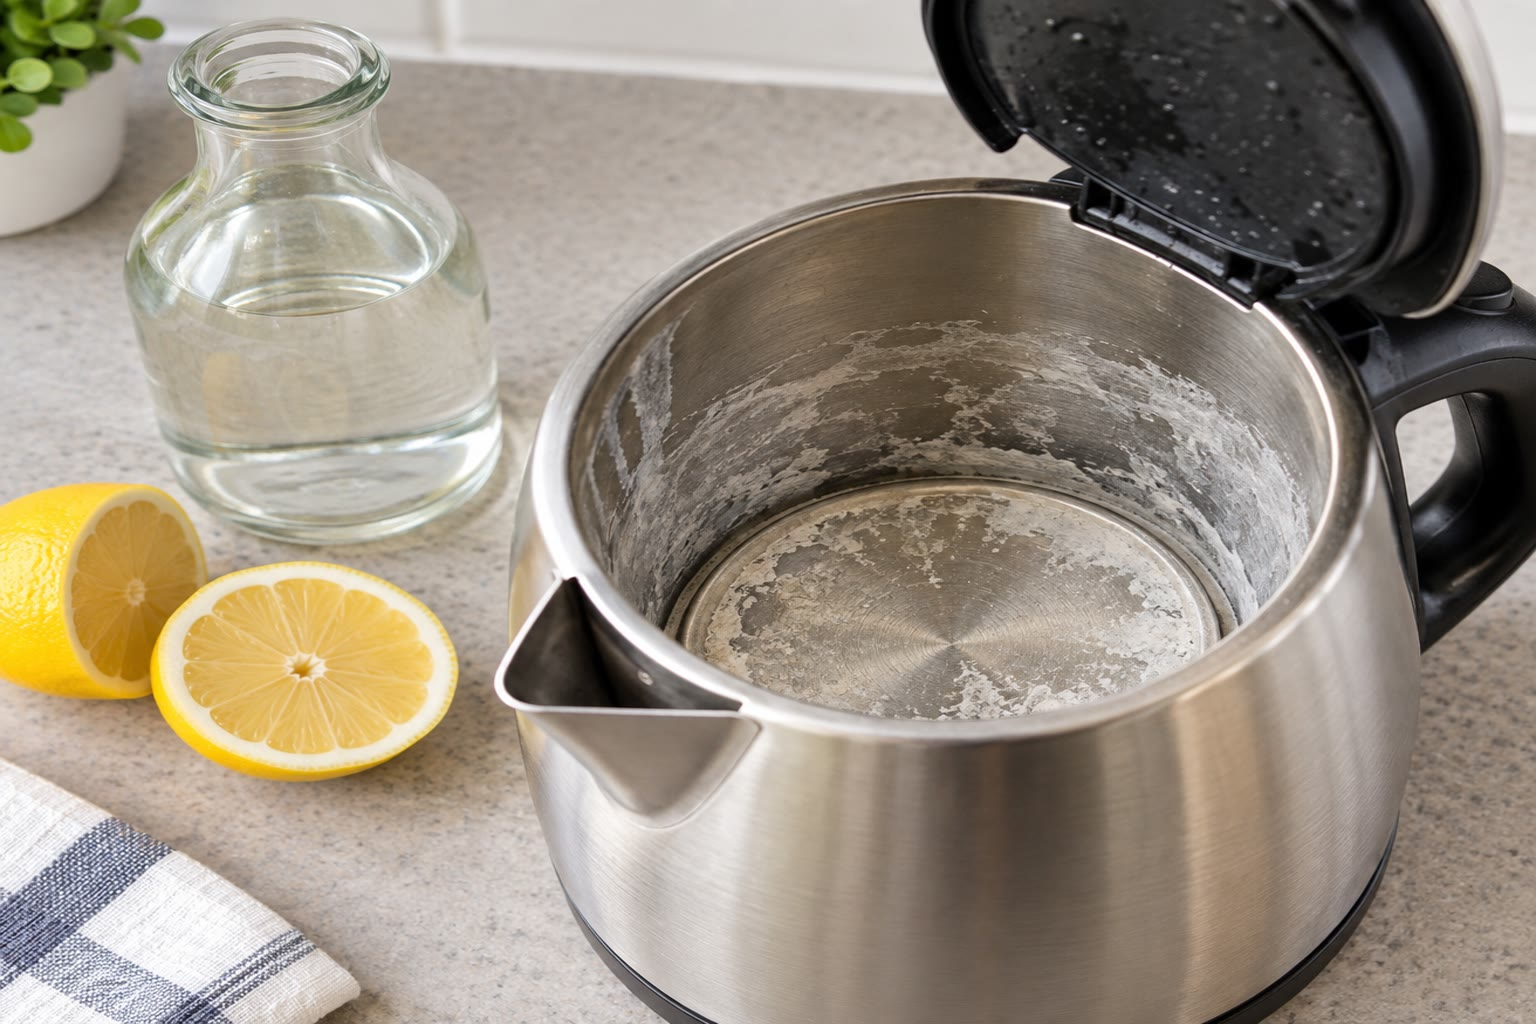
\includegraphics[width=0.5\linewidth]{images/book2/ai/b1-10-descaling.jpg}

{\small ترسبات الكلس، أي كربونات الكالسيوم، في غلاية. تتفاعل \omterm{def:b1:predominant-reaction:strong-acid}{الأحماض الضعيفة} في
الخل وعصير الليمون مع أيون الكربونات فتذيبه.}
\end{omfigure}

\section{مزدوجات برونستد والرقم الهيدروجيني}

\begin{definition}[حمض برونستد وقاعدته، المزدوجة]\label{def:b1:predominant-reaction:bronsted}
\emph{حمض برونستد}\index{حمض برونستد} نوع كيميائي قادر على منح
بروتون \ce{H+}؛ و\emph{قاعدة برونستد}\index{قاعدة برونستد} نوع
قادر على تقبّله. والحمض HA والقاعدة A التي يصير إليها بفقد
بروتون يكوّنان \emph{مزدوجة حمض/قاعدة}\index{مزدوجة حمض/قاعدة} HA/A،
تربطهما نصف المعادلة الشكلية $\mathrm{HA} \rightleftharpoons
\mathrm{A} + \ce{H+}$. وفي الماء لا يكون البروتون حرًا أبدًا: بل يحمله
جزيء ماء على هيئة \ce{H3O+}.
\end{definition}

\begin{definition}[الأمفوليت]\label{def:b1:predominant-reaction:ampholyte}
\emph{الأمفوليت}\index{أمفوليت} (أو النوع المذبذب) هو قاعدة
مزدوجة وحمض مزدوجة أخرى: الماء ($\ce{H3O+}/\ce{H2O}$
و$\ce{H2O}/\ce{OH-}$)، وأيون الهيدروجينوكربونات ($\ce{CO2,H2O}/\ce{HCO3-}$
و$\ce{HCO3-}/\ce{CO3^{2-}}$)، وأيون ثنائي هيدروجين الفوسفات.
\end{definition}

\begin{definition}[التحلل البروتوني الذاتي، الجداء الأيوني، الرقم الهيدروجيني]\label{def:b1:predominant-reaction:autoprotolysis}
يخضع الماء \emph{للتحلل البروتوني الذاتي}\index{تحلل بروتوني ذاتي}،
\ce{2H2O <=> H3O+ + OH-}، الذي ثابته $K_e = [\ce{H3O+}][\ce{OH-}]$ هو
\emph{الجداء الأيوني للماء}\index{الجداء الأيوني للماء}؛ وعند
\qty{25}{\celsius}، $K_e = 10^{-14.00}$، فيكون $\mathrm{p}K_e = 14.00$. والرقم الهيدروجيني
لمحلول هو $\mathrm{pH} = -\log a(\ce{H3O+}) \approx -\log[\ce{H3O+}]$.
ويكون المحلول متعادلًا حين $[\ce{H3O+}] = [\ce{OH-}]$، أي عند
$\mathrm{pH} = \mathrm{p}K_e/2 = 7.00$ في \qty{25}{\celsius}.
% ledger: dfg:H2O_l, dfg:OH-_ao (pKe computed in figdata/bachelor-1/aqueous-constants.py)
\end{definition}

\section{القوة: \texorpdfstring{$K_a$}{Ka} و\texorpdfstring{\babelsublr{p$K_a$}}{pKa} وتأثير التسوية}

\begin{definition}[ثابت الحمضية]\label{def:b1:predominant-reaction:acidity-constant}
\emph{ثابت الحمضية}\index{ثابت الحمضية} لمزدوجة HA/A هو
ثابت تفاعل الحمض مع الماء،
\[
  \mathrm{HA} + \ce{H2O} \rightleftharpoons \mathrm{A} + \ce{H3O+}, \qquad
  K_a = \frac{[\mathrm{A}][\ce{H3O+}]}{[\mathrm{HA}]}, \qquad
  \mathrm{p}K_a = -\log K_a .
\]
وكلما كبر $K_a$ (أي صغر $\mathrm{p}K_a$) كان الحمض أقوى
وقاعدته المرافقة أضعف.
\end{definition}

\begin{definition}[الأحماض والقواعد القوية والضعيفة]\label{def:b1:predominant-reaction:strong-acid}
يكون الحمض \emph{قويًا}\index{حمض قوي} في الماء إذا كان تفاعله مع
الماء تامًا: فلا يبقى أي جزيء HA (حمض الكلوريدريك، وحمض النتريك، وحمض
البيركلوريك، والحمضية الأولى لحمض الكبريتيك)؛ وإلا فهو
\emph{ضعيف}\index{حمض ضعيف}. وتكون القاعدة \emph{قوية}\index{قاعدة قوية}
إذا كان تفاعلها مع الماء تامًا، معطيًا \ce{OH-} (الهيدروكسيدات،
وأيون الأكسيد، والألكوكسيدات)، و\emph{ضعيفة}\index{قاعدة ضعيفة} في الحالة الأخرى.
\end{definition}

\begin{definition}[تأثير التسوية]\label{def:b1:predominant-reaction:levelling}
في الماء، يتفاعل كل حمض أقوى من \ce{H3O+} تفاعلًا تامًا ليعطي
\ce{H3O+}، وكل قاعدة أقوى من \ce{OH-} تفاعلًا تامًا لتعطي
\ce{OH-}: فلا يمكن التمييز بين قواها. هذا هو
\emph{تأثير التسوية}\index{تأثير التسوية} للمذيب. وللأحماض
\omterm{def:b1:predominant-reaction:strong-acid}{والقواعد الضعيفة} في الماء $0 < \mathrm{p}K_a < 14$، إذ تحدّ السلّمَ
مزدوجتا الماء
نفسه ($\mathrm{p}K_a(\ce{H3O+}/\ce{H2O}) = 0$
و$\mathrm{p}K_a(\ce{H2O}/\ce{OH-}) = 14$).
\end{definition}

\begin{center}
\small
\begin{tabular}{lll@{\hspace{2.5em}}lll}
\hline
المزدوجة & \babelsublr{p$K_a$} & & المزدوجة & \babelsublr{p$K_a$} & \\
\hline
$\ce{HSO4-}/\ce{SO4^{2-}}$ & 1.99 & & $\ce{CO2,H2O}/\ce{HCO3-}$ & 6.37 & \\
$\ce{H3PO4}/\ce{H2PO4-}$ & 2.15 & & $\ce{H2PO4-}/\ce{HPO4^{2-}}$ & 7.21 & \\
$\ce{HF}/\ce{F-}$ & 3.16 & & $\ce{HClO}/\ce{ClO-}$ & 7.55 & \\
$\ce{HCOOH}/\ce{HCOO-}$ & 3.74 & & $\ce{NH4+}/\ce{NH3}$ & 9.25 & \\
$\ce{CH3COOH}/\ce{CH3COO-}$ & 4.76 & & $\ce{C6H5OH}/\ce{C6H5O-}$ & 9.99 & \\
$\ce{C6H5NH3+}/\ce{C6H5NH2}$ & 4.60 & & $\ce{HCO3-}/\ce{CO3^{2-}}$ & 10.33 & \\
$\ce{C6H5COOH}/\ce{C6H5COO-}$ & 4.21 & & $\ce{CH3NH3+}/\ce{CH3NH2}$ & 10.66 & \\
\hline
\end{tabular}
\end{center}
% ledger: pka:methanoic, pka:ethanoic, pka:anilinium, pka:benzoic,
% pka:phenol, pka:methylammonium (IUPAC dataset); dfg:HSO4-_ao,
% dfg:SO42-_ao, dfg:H3PO4_ao, dfg:H2PO4-_ao, dfg:HPO42-_ao, dfg:HF_ao,
% dfg:F-_ao, dfg:CO2_ao, dfg:HCO3-_ao, dfg:CO32-_ao, dfg:HClO_ao,
% dfg:ClO-_ao, dfg:NH4+_ao, dfg:NH3_ao (pKa computed from NBS-82)

\section{مخططات الغلبة والتوزيع}

\begin{definition}[مخططا الغلبة والتوزيع]\label{def:b1:predominant-reaction:predominance}
من أجل مزدوجة HA/A، $\mathrm{pH} = \mathrm{p}K_a + \log([\mathrm{A}]/[\mathrm{HA}])$:
فيغلب الحمض ($[\mathrm{HA}] > [\mathrm{A}]$) من أجل
$\mathrm{pH} < \mathrm{p}K_a$، وتغلب القاعدة من أجل $\mathrm{pH} > \mathrm{p}K_a$.
و\emph{مخطط الغلبة}\index{مخطط الغلبة} هو محور pH
مقسَّمًا عند كل $\mathrm{p}K_a$ إلى المناطق التي يغلب فيها كل
شكل. و\emph{مخطط التوزيع}\index{مخطط التوزيع}
يعطي كسر كل شكل، $[\text{الشكل}]/C$، بدلالة pH.
\end{definition}

\begin{proposition}[علاقة هندرسون والكسور]\label{prop:b1:predominant-reaction:henderson}
من أجل مزدوجة HA/A تركيزها الكلي $C = [\mathrm{HA}] + [\mathrm{A}]$،
\[
  \mathrm{pH} = \mathrm{p}K_a + \log\frac{[\mathrm{A}]}{[\mathrm{HA}]}, \qquad
  \frac{[\mathrm{HA}]}{C} = \frac{1}{1 + 10^{\mathrm{pH} - \mathrm{p}K_a}}, \qquad
  \frac{[\mathrm{A}]}{C} = \frac{1}{1 + 10^{\mathrm{p}K_a - \mathrm{pH}}} .
\]
فعلى بعد وحدة pH واحدة من $\mathrm{p}K_a$ يكون الشكل الثانوي دون
10\,\% من المجموع؛ وعلى بعد وحدتين، دون 1\,\%.
\end{proposition}

\begin{proof}
نأخذ لوغاريتم $K_a = [\mathrm{A}][\ce{H3O+}]/[\mathrm{HA}]$. فيكون
$[\mathrm{A}]/[\mathrm{HA}] = 10^{\mathrm{pH}-\mathrm{p}K_a}$، وبقسمة
$[\mathrm{HA}]$ على $[\mathrm{HA}] + [\mathrm{A}]$ نحصل على الكسور. وعند
$\mathrm{pH} = \mathrm{p}K_a + 1$، $[\mathrm{HA}]/C = 1/11 < 10\,\%$؛ وعند
$+2$، $1/101$.
\end{proof}

\begin{omfigure}
\begin{tikzpicture}
\begin{axis}[name=e,
  width=0.48\linewidth, height=5.2cm, xmin=0, xmax=14, ymin=0, ymax=1.05,
  axis x line=bottom, axis y line=left, xlabel={\babelsublr{pH}}, ylabel={الكسر},
  xtick={0,2,4,6,8,10,12,14},
  tick label style={font=\small}, label style={font=\small}]
\addplot[omDef, thick] table[x=pH, y=HA] {figdata/out/bachelor-1-distribution-diagrams-ethanoic.dat};
\addplot[omThm, thick] table[x=pH, y=A] {figdata/out/bachelor-1-distribution-diagrams-ethanoic.dat};
\draw[dotted] (axis cs:4.76,0) -- (axis cs:4.76,0.5);
\node[omDef, font=\footnotesize, anchor=west] at (axis cs:0.3,0.3) {\ce{CH3COOH}};
\node[omThm, font=\footnotesize, anchor=east] at (axis cs:13.7,0.3) {\ce{CH3COO-}};
\node[font=\small, anchor=north west] at (axis cs:4.8,0.48) {4.76};
\end{axis}
\begin{axis}[at={(e.east)}, anchor=west, xshift=1.1cm,
  width=0.48\linewidth, height=5.2cm, xmin=0, xmax=14, ymin=0, ymax=1.05,
  axis x line=bottom, axis y line=left, xlabel={\babelsublr{pH}}, ylabel={الكسر},
  xtick={0,2,4,6,8,10,12,14},
  legend style={font=\scriptsize, draw=none, at={(0.5,1.04)}, anchor=south, legend columns=4},
  tick label style={font=\small}, label style={font=\small}]
\addplot[omDef, thick] table[x=pH, y=H3A] {figdata/out/bachelor-1-distribution-diagrams-phosphoric.dat};
\addplot[omMeth, thick] table[x=pH, y=H2A] {figdata/out/bachelor-1-distribution-diagrams-phosphoric.dat};
\addplot[omProp, thick] table[x=pH, y=HA] {figdata/out/bachelor-1-distribution-diagrams-phosphoric.dat};
\addplot[omThm, thick] table[x=pH, y=A] {figdata/out/bachelor-1-distribution-diagrams-phosphoric.dat};
\legend{\ce{H3PO4}, \ce{H2PO4-}, \ce{HPO4^{2-}}, \ce{PO4^{3-}}}

\end{axis}
\end{tikzpicture}

\begin{tikzpicture}[font=\small, >={Stealth}]
  \draw[->, thick] (0,0) -- (14.2*0.85,0) node[right] {pH};
  \foreach \x/\l in {2.15/2.15, 7.21/7.21, 12.34/12.34}
    \draw (\x*0.85,0.15) -- (\x*0.85,-0.15) node[below] {\l};
  \node[above] at (1.07*0.85,0.1) {\ce{H3PO4}};
  \node[above] at (4.68*0.85,0.1) {\ce{H2PO4-}};
  \node[above] at (9.78*0.85,0.1) {\ce{HPO4^{2-}}};
  \node[above] at (13.3*0.85,0.1) {\ce{PO4^{3-}}};
\end{tikzpicture}

{\small مخططا التوزيع لحمض الإيثانويك (يسارًا) ولحمض الفوسفوريك
(يمينًا)، \omterm{def:b1:predominant-reaction:predominance}{ومخطط الغلبة} لحمض الفوسفوريك. كل تقاطع
لمنحنيين متجاورين يقع عند $\mathrm{p}K_a$؛ والأمفوليتان
\ce{H2PO4-} و\ce{HPO4^{2-}} يكادان يكونان الشكل الوحيد في منتصف
منطقتيهما.}
\end{omfigure}

\section{طريقة التفاعل الغالب}

\begin{proposition}[ثابت تفاعل حمض--قاعدة]\label{prop:b1:predominant-reaction:k-of-reaction}
تفاعل الحمض $\mathrm{HA}_1$ لمزدوجة مع القاعدة
$\mathrm{A}_2$ لمزدوجة أخرى،
$\mathrm{HA}_1 + \mathrm{A}_2 \rightleftharpoons \mathrm{A}_1 + \mathrm{HA}_2$،
ثابته
\[
  K = \frac{K_{a1}}{K_{a2}} = 10^{\,\mathrm{p}K_{a2} - \mathrm{p}K_{a1}} .
\]
وهو مواتٍ ($K > 1$) حين يكون الحمض أقوى من الحمض الذي
يتكوّن ($\mathrm{p}K_{a1} < \mathrm{p}K_{a2}$)، وكمّي (بالمعنى
الوارد في \cref{met:b1:extent-q-and-k:quantitative}) حين يتجاوز الفرق
بين $\mathrm{p}K_a$ نحو 4.
\end{proposition}

\begin{proof}
التفاعل هو مجموع $\mathrm{HA}_1 + \ce{H2O} \rightleftharpoons
\mathrm{A}_1 + \ce{H3O+}$ ($K_{a1}$) وعكس $\mathrm{HA}_2 +
\ce{H2O} \rightleftharpoons \mathrm{A}_2 + \ce{H3O+}$ ($1/K_{a2}$)؛
فتعطي \cref{prop:b1:extent-q-and-k:combine-k} $K = K_{a1}/K_{a2}$.
\end{proof}

\begin{definition}[التفاعل الغالب، المحلول المكافئ]\label{def:b1:predominant-reaction:predominant-reaction}
في محلول يحوي عدة أحماض وقواعد، يكون \emph{التفاعل
الغالب}\index{تفاعل غالب} هو التفاعل ذا الثابت الأكبر
بين أقوى حمض وأقوى قاعدة حاضرين. وحين يكون
\omterm{def:b1:extent-q-and-k:quantitative}{كمّيًا} يُعامَل على أنه تام، ويُستبدل بالمحلول
\emph{المحلولُ المكافئ}\index{محلول مكافئ}: أي المحلول
الذي نحصل عليه بعد اكتمال هذا التفاعل، والذي له pH المحلول
الحقيقي نفسه.
\end{definition}

\begin{method}[طريقة التفاعل الغالب]\label{met:b1:predominant-reaction:method}
لإيجاد pH محلول وتركيبه:
\begin{enumerate}
  \item عدّد الأنواع المُدخلة (والماء) وضع مزدوجاتها
        على سلّم $\mathrm{p}K_a$، الأحماض في جهة والقواعد في الأخرى؛
  \item أوجد أقوى حمض وأقوى قاعدة حاضرين؛
  \item إن كان ثابت تفاعلهما كبيرًا ($K > 10^4$، أو
        $\Delta\mathrm{p}K_a > 4$)، فعامل التفاعل على أنه تام واكتب
        \omterm{def:b1:predominant-reaction:predominant-reaction}{المحلول المكافئ}؛ ثم عد إلى الخطوة 2؛
  \item حين يكون ثابت \omterm{def:b1:predominant-reaction:predominant-reaction}{التفاعل الغالب} صغيرًا، فهو الذي يحدد
        pH: اكتب جدول تقدمه وحلّ $Q = K$، عادةً بفرضية
        أن تقدمه صغير؛
  \item تحقق من الفرضيات: الأنواع الثانوية ثانوية حقًا،
        والتفاعلات الأخرى (ومنها \omterm{def:b1:predominant-reaction:autoprotolysis}{التحلل البروتوني الذاتي} للماء)
        مهملة.
\end{enumerate}
\end{method}

\begin{omfigure}
\begin{tikzpicture}[font=\small, >={Stealth}]
  \draw[->, thick] (0,-0.3) -- (0,7.6) node[above] {p$K_a$};
  \foreach \y/\a/\b in {0/\ce{H3O+}/\ce{H2O}, 1.58/\ce{HF}/\ce{F-}, 2.38/\ce{CH3COOH}/\ce{CH3COO-},
      3.62/\ce{H2PO4-}/\ce{HPO4^{2-}}, 4.62/\ce{NH4+}/\ce{NH3}, 7/\ce{H2O}/\ce{OH-}} {
    \draw (-0.12,\y) -- (0.12,\y);
    \node[anchor=east] at (-0.2,\y) {\a};
    \node[anchor=west] at (0.2,\y) {\b};
  }
  \foreach \y/\l in {0/0, 1.58/3.16, 2.38/4.76, 3.62/7.21, 4.62/9.25, 7/14} \node[black!60, anchor=west] at (3.0,\y) {\l};
  \draw[->, omThm, thick] (-1.6,2.55) -- (1.2,4.45);
  \node[omThm, anchor=west, align=left] at (4.2,3.5) {يتفاعل الحمض مع كل\\\foreignlanguage{arabic}{قاعدة تقع فوقه: $K > 1$}};
  \node[anchor=south] at (-1.4,7.35) {الأحماض};
  \node[anchor=south] at (1.2,7.35) {القواعد};
\end{tikzpicture}

{\small سلّم $\mathrm{p}K_a$ (مرسوم وقيم \babelsublr{p$K_a$} تتزايد صعودًا؛
والقيم على اليمين). يتفاعل الحمض تفاعلًا مواتيًا مع كل قاعدة تقع
فوقه على السلّم: هنا حمض الإيثانويك مع الأمونيا،
$K = 10^{9.25 - 4.76} = 10^{4.49}$.}
\end{omfigure}

\begin{proposition}[pH المحاليل البسيطة]\label{prop:b1:predominant-reaction:ph-formulas}
عند التركيز $C$ (بالوحدة \unit{mol/L})، مع $\mathrm{p}C = -\log C$:
\begin{itemize}
  \item \omterm{def:b1:predominant-reaction:strong-acid}{الحمض القوي}: $\mathrm{pH} = \mathrm{p}C$، صالحة من أجل
        $\mathrm{pH} < 6.5$؛
  \item \omterm{def:b1:predominant-reaction:strong-acid}{الحمض الضعيف} القليل التفكك: $\mathrm{pH} = \frac12(\mathrm{p}K_a
        + \mathrm{p}C)$، صالحة إذا كان $\mathrm{pH} < \mathrm{p}K_a - 1$؛
  \item \omterm{def:b1:predominant-reaction:strong-acid}{القاعدة الضعيفة} القليلة البرتنة: $\mathrm{pH} = \frac12(\mathrm{p}K_e +
        \mathrm{p}K_a - \mathrm{p}C)$، صالحة إذا كان $\mathrm{pH} > \mathrm{p}K_a +
        1$؛
  \item \omterm{def:b1:predominant-reaction:ampholyte}{الأمفوليت} مع $\mathrm{p}K_{a2} - \mathrm{p}K_{a1} > 4$:
        $\mathrm{pH} = \frac12(\mathrm{p}K_{a1} + \mathrm{p}K_{a2})$،
        أيًّا كان $C$ (إن لم يكن مخففًا جدًا).
\end{itemize}
\end{proposition}

\begin{proof}
\omterm{def:b1:predominant-reaction:strong-acid}{الحمض القوي}: \ce{HA + H2O -> A- + H3O+} تام، $[\ce{H3O+}] = C$،
وإسهام الماء نفسه ($10^{-7}$) مهمل إذا كان $C > 10^{-6.5}$.
\omterm{def:b1:predominant-reaction:strong-acid}{الحمض الضعيف}: \omterm{def:b1:predominant-reaction:predominant-reaction}{التفاعل الغالب} هو $\mathrm{HA} + \ce{H2O}
\rightleftharpoons \mathrm{A} + \ce{H3O+}$ بتقدم $x = [\ce{H3O+}]
= [\mathrm{A}]$؛ وإذا كان $x \ll C$، فإن $K_a = x^2/C$، $\mathrm{pH} = \frac12(\mathrm{p}K_a
+ \mathrm{p}C)$؛ والفرضية $[\mathrm{A}] < [\mathrm{HA}]/10$ هي
$\mathrm{pH} < \mathrm{p}K_a - 1$. \omterm{def:b1:predominant-reaction:strong-acid}{القاعدة الضعيفة}: الشيء نفسه مع $\mathrm{A} +
\ce{H2O} \rightleftharpoons \mathrm{HA} + \ce{OH-}$، الذي ثابته $K_e/K_a$.
\omterm{def:b1:predominant-reaction:ampholyte}{الأمفوليت} \babelsublr{HA$^-$}: \omterm{def:b1:predominant-reaction:predominant-reaction}{التفاعل الغالب} هو $2\,\mathrm{HA}^- \rightleftharpoons
\mathrm{H_2A} + \mathrm{A}^{2-}$، فيكون $[\mathrm{H_2A}] = [\mathrm{A}^{2-}]$؛
وبضرب $K_{a1} = [\mathrm{HA}^-]h/[\mathrm{H_2A}]$ في $K_{a2} =
[\mathrm{A}^{2-}]h/[\mathrm{HA}^-]$ نحصل على $h^2 = K_{a1}K_{a2}$.
\end{proof}

\begin{omfigure}
\begin{tikzpicture}
\begin{axis}[
  width=0.66\linewidth, height=5.6cm, xmin=0, xmax=8, ymin=0, ymax=8,
  axis x line=bottom, axis y line=left,
  xlabel={\babelsublr{$\mathrm{p}C = -\log C$}}, ylabel={\babelsublr{pH}},
  xtick={0,1,2,3,4,5,6,7,8}, ytick={0,1,2,3,4,5,6,7,8},
  tick label style={font=\small}, label style={font=\small},
  legend style={font=\small, draw=none, at={(0.02,0.98)}, anchor=north west}]
\addplot[omDef, very thick] table[x=pC, y=pH] {figdata/out/bachelor-1-weak-acid-ph.dat};
\addplot[omProp, dashed] table[x=pC, y=weak] {figdata/out/bachelor-1-weak-acid-ph.dat};
\addplot[black!50, dotted, thick] table[x=pC, y=strong] {figdata/out/bachelor-1-weak-acid-ph.dat};
\draw[black!30] (axis cs:0,7) -- (axis cs:8,7);
\legend{{القيمة الدقيقة}, $\frac12(\mathrm{p}K_a + \mathrm{p}C)$, $\mathrm{pH} = \mathrm{p}C$}
\end{axis}
\end{tikzpicture}

{\small pH محاليل حمض الإيثانويك بدلالة $\mathrm{p}C$، محسوبًا
حسابًا دقيقًا من حصيلة الشحنات. فالحمض المركز قليل
التفكك ويتبع $\frac12(\mathrm{p}K_a + \mathrm{p}C)$؛ وإذا خُفف
دون نحو $10^{-6}$ mol/L تفكك كليًا وسلك سلوك
\omterm{def:b1:predominant-reaction:strong-acid}{حمض قوي}؛ وفي التخفيف الشديد جدًا يؤول pH إلى 7.}
\end{omfigure}

\begin{example}[حمض الإيثانويك والأمونيا]\label{ex:b1:predominant-reaction:mixture}
لنخلط \qty{0.10}{mol} من حمض الإيثانويك و\qty{0.10}{mol} من الأمونيا في
\qty{1.0}{L}. أقوى حمض هو \ce{CH3COOH}، وأقوى قاعدة
\ce{NH3}: \ce{CH3COOH + NH3 <=> CH3COO- + NH4+}، $K = 10^{9.25 - 4.76} =
10^{4.49}$، تفاعل كمّي. ويحوي \omterm{def:b1:predominant-reaction:predominant-reaction}{المحلول المكافئ}
\qty{0.10}{mol/L} من \ce{CH3COO-} ومن \ce{NH4+}. وتفاعله
الغالب، \ce{NH4+ + CH3COO- <=> NH3 + CH3COOH}، ثابته صغير
$10^{-4.49}$ ويُبقي $[\ce{NH3}] = [\ce{CH3COOH}]$، ومنه، كما في
\omterm{def:b1:predominant-reaction:ampholyte}{الأمفوليت}، $\mathrm{pH} = \frac12(4.76 + 9.25) = 7.01$.
\end{example}

\section{الأحماض المتعددة البروتونات والمحاليل المنظمة}

\begin{definition}[الحمض المتعدد البروتونات]\label{def:b1:predominant-reaction:polyprotic}
\emph{الحمض المتعدد البروتونات}\index{حمض متعدد البروتونات} يستطيع أن يمنح عدة بروتونات
على التوالي، ولكل خطوة ثابتها: حمض الفوسفوريك
\ce{H3PO4} ($\mathrm{p}K_a$ = 2.15، 7.21، 12.34)، وحمض الكربونيك
(\ce{CO2,H2O}؛ 6.37، 10.33)، وحمض الكبريتيك (حمضيته الأولى قوية، والثانية
1.99). وتتزايد قيم $\mathrm{p}K_a$ المتتالية: فنزع بروتون من
نوع سالب الشحنة أصلًا يكلّف أكثر.
\end{definition}

\begin{example}[حمض الفوسفوريك عند \texorpdfstring{\qty{0.10}{mol/L}}{0.10 mol/L}]\label{ex:b1:predominant-reaction:h3po4}
\omterm{def:b1:predominant-reaction:predominant-reaction}{التفاعل الغالب} هو الحمضية الأولى. مع $x = [\ce{H3O+}]$،
$x^2/(0.10 - x) = 10^{-2.15}$؛ وهنا ليس $x$ صغيرًا مقارنةً بالتركيز $C$،
فتُحل المعادلة التربيعية $x^2 + K_{a1}x - K_{a1}C = 0$: $x =
\qty{0.0233}{mol/L}$، $\mathrm{pH} = 1.63$. أما الحمضية الثانية
($\mathrm{p}K_{a2} = 7.21$) فلا تسهم بشيء عند هذا pH.
\end{example}

\begin{definition}[المحلول المنظم]\label{def:b1:predominant-reaction:buffer}
\emph{المحلول المنظم}\index{محلول منظم} محلول يتغير pH
قليلًا حين تضاف إليه كمية صغيرة من حمض أو قاعدة، أو حين
يُخفَّف. والمحلول المنظم المعتاد خليط من \omterm{def:b1:predominant-reaction:strong-acid}{حمض ضعيف} وقاعدته المرافقة
بكميتين متقاربتين؛ ويكون pH قريبًا من $\mathrm{p}K_a$
المزدوجة.
\end{definition}

\begin{proposition}[لماذا يقاوم المحلول المنظم]\label{prop:b1:predominant-reaction:buffer}
من أجل \omterm{def:b1:predominant-reaction:buffer}{محلول منظم} من $n_a$ مول من الحمض و$n_b$ مول من القاعدة، لا يتعلق $\mathrm{pH} =
\mathrm{p}K_a + \log(n_b/n_a)$ بالحجم. وإضافة
$\delta$ مول من \omterm{def:b1:predominant-reaction:strong-acid}{حمض قوي} تغيّره بمقدار
\[
  \Delta\mathrm{pH} = \log\frac{n_b - \delta}{n_a + \delta} - \log\frac{n_b}{n_a}
  \approx -\frac{\delta}{\ln 10}\left(\frac{1}{n_a} + \frac{1}{n_b}\right),
\]
وهو أصغر ما يكون حين $n_a = n_b$ عند كمية كلية معطاة.
\end{proposition}

\begin{proof}
يتفاعل \omterm{def:b1:predominant-reaction:strong-acid}{الحمض القوي} تفاعلًا تامًا مع القاعدة: $n_b \to n_b - \delta$،
$n_a \to n_a + \delta$. ومشتقة $f(\delta) = \log(n_b - \delta) -
\log(n_a + \delta)$ عند 0 هي $-\frac{1}{\ln10}\big(\frac{1}{n_b} +
\frac{1}{n_a}\big)$؛ ومن أجل $n_a + n_b$ ثابت، يكون $\frac1{n_a} + \frac1{n_b}$
أصغر ما يكون حين $n_a = n_b$.
\end{proof}

\begin{definition}[درجة التفكك]\label{def:b1:predominant-reaction:dissociation}
\emph{درجة التفكك}\index{درجة التفكك} \omterm{def:b1:predominant-reaction:strong-acid}{لحمض ضعيف}
HA تركيزه التحليلي $C$ هي $\alpha = [\mathrm{A}]/C$، أي
كسر الحمض الذي فككه الماء؛ وهي تحقق قانون التخفيف لأوستفالد
$\alpha^2C/(1 - \alpha) = K_a$، وتؤول إلى 1 عندما $C \to 0$.
\end{definition}

\begin{inthelab}[تحضير محلول منظم]
يُحضَّر \omterm{def:b1:predominant-reaction:buffer}{المحلول المنظم} في المختبر بوزن الحمض وملحه
(مثلًا ثنائي هيدروجين فوسفات الصوديوم وهيدروجين فوسفات
ثنائي الصوديوم)، أو بإضافة حجم مقيس من محلول هيدروكسيد الصوديوم
إلى الحمض مع قراءة مقياس pH معايَر مسبقًا بمحلولين
منظمين معياريين؛ ثم يُكمَل المحلول إلى العلامة في
حوجلة معيارية.
\end{inthelab}

\section{تمارين}

\begin{exercise}[$\star$]\label{exo:b1:predominant-reaction:1}
اكتب القاعدة المرافقة لكل من \ce{H2SO4} و\ce{HCO3-} و\ce{NH4+}
و\ce{H2O}، والحمض المرافق لكل من \ce{NH3} و\ce{HPO4^{2-}} و\ce{OH-}
و\ce{H2O}. أي هذه الأنواع \omterm{def:b1:predominant-reaction:ampholyte}{أمفوليتات}؟
\end{exercise}

\begin{exercise}[$\star$]\label{exo:b1:predominant-reaction:2}
مستعينًا بجدول قيم $\mathrm{p}K_a$، رتّب حمض الهيدروفلوريك وحمض الإيثانويك
وأيون الأمونيوم وحمض الهيبوكلوروز بحسب القوة، وأعطِ $K_a$ لكل
منها.
\end{exercise}

\begin{exercise}[$\star$]\label{exo:b1:predominant-reaction:3}
احسب pH محلول تركيزه \qty{0.010}{mol/L} من حمض الكلوريدريك،
وpH محلول تركيزه \qty{0.010}{mol/L} من هيدروكسيد الصوديوم، عند
\qty{25}{\celsius}.
\end{exercise}

\begin{exercise}[$\star$]\label{exo:b1:predominant-reaction:4}
ارسم \omterm{def:b1:predominant-reaction:predominance}{مخطط الغلبة} للمزدوجة $\ce{CH3COOH}/\ce{CH3COO-}$.
أي الشكلين يغلب في مشروب غازي ذي pH يساوي 3، وفي الدم ذي pH يساوي 7.4؟ وما
كسر الحمض الموجود في الشكل الحمضي عند pH 3.76؟
\end{exercise}

\begin{exercise}[$\star\star$]\label{exo:b1:predominant-reaction:5}
احسب pH محلول أمونيا تركيزه \qty{0.10}{mol/L} وتحقق من
الفرضية المعتمدة.
\end{exercise}

\begin{exercise}[$\star\star$]\label{exo:b1:predominant-reaction:6}
احسب pH محلول حمض الإيثانويك تركيزه \qty{0.010}{mol/L}
\omterm{def:b1:predominant-reaction:dissociation}{ودرجة التفكك}؛ وتحقق من الفرضية.
\end{exercise}

\begin{exercise}[$\star\star$]\label{exo:b1:predominant-reaction:7}
اكتب \omterm{def:b1:predominant-reaction:predominant-reaction}{التفاعل الغالب} وثابته وpH المحلول
الناتج عن خلط \qty{0.10}{mol} من حمض الهيدروفلوريك
و\qty{0.050}{mol} من هيدروكسيد الصوديوم في \qty{1.0}{L}.
\end{exercise}

\begin{exercise}[$\star\star$]\label{exo:b1:predominant-reaction:8}
يحوي \omterm{def:b1:predominant-reaction:buffer}{محلول منظم} \qty{0.050}{mol} من حمض الإيثانويك و\qty{0.050}{mol}
من إيثانوات الصوديوم في \qty{1.0}{L}. احسب pH، ثم pH بعد
إضافة \qty{0.010}{mol} من حمض الكلوريدريك. وقارن بالإضافة نفسها
إلى \qty{1.0}{L} من الماء النقي.
\end{exercise}

\begin{exercise}[$\star\star$]\label{exo:b1:predominant-reaction:9}
لحمضي الكلوريدريك والنتريك القوة نفسها في الماء، لكن ليس في
حمض الإيثانويك النقي مذيبًا. فسّر، وبيّن ما أقوى حمض
يمكن أن يوجد في الماء.
\end{exercise}

\begin{exercise}[$\star\star\star$]\label{exo:b1:predominant-reaction:10}
احسب pH محلول كربونات الصوديوم تركيزه \qty{0.10}{mol/L}،
وتحقق من أن القاعدية الثانية يمكن إهمالها.
\end{exercise}

\begin{exercise}[$\star\star\star$]\label{exo:b1:predominant-reaction:11}
برهن على قانون التخفيف لأوستفالد واحسب \omterm{def:b1:predominant-reaction:dissociation}{درجة تفكك}
حمض الإيثانويك عند $C = \qty{1.0e-3}{mol/L}$. لماذا يخفق
التقريب $\alpha \ll 1$ هنا؟
\end{exercise}

\begin{exercise}[$\star\star\star$]\label{exo:b1:predominant-reaction:12}
يحوي محلول \qty{0.010}{mol/L} من حمض الكلوريدريك
و\qty{0.10}{mol/L} من حمض الإيثانويك. أوجد pH وتركيز
أيونات الإيثانوات؛ وفسّر لماذا لا يكاد \omterm{def:b1:predominant-reaction:strong-acid}{الحمض الضعيف} يتفكك.
\end{exercise}

\section{مسألة: محلول منظم بالفوسفات لمختبر زراعة الخلايا}

\begin{problem}[{مسألة نهاية الأسبوع --- الحمضيات الثلاث لحمض
الفوسفوريك، وpH أملاحه الصوديومية الثلاثة، والمحاليل المكافئة،
وحجم هيدروكسيد الصوديوم الذي يعطي محلولًا منظمًا ذا pH يساوي 7.20}]
\label{pb:b1:predominant-reaction:1}
تحتاج الخلايا المستنبَتة في المختبر إلى وسط ذي pH قريب من 7.2. معطيات عند
\qty{25}{\celsius}: قيم $\mathrm{p}K_a$ لحمض الفوسفوريك 2.15 و7.21
و12.34؛ $\mathrm{p}K_e = 14.00$.

\medskip
\noindent\textbf{الجزء الأول --- حمض الفوسفوريك.}
\begin{enumerate}
  \item اكتب المزدوجات الثلاث وأنصاف معادلاتها.
  \item ارسم \omterm{def:b1:predominant-reaction:predominance}{مخطط الغلبة} لحمض الفوسفوريك.
  \item أي نوع يغلب عند pH 1 و5 و9 و13؟
  \item أي الأنواع \omterm{def:b1:predominant-reaction:ampholyte}{أمفوليتات}؟
  \item لماذا كانت كل قيمة $\mathrm{p}K_a$ أكبر من سابقتها؟
\end{enumerate}

\medskip
\noindent\textbf{الجزء الثاني --- ثلاثة محاليل عند \qty{0.100}{mol/L}.}
\begin{enumerate}[resume]
  \item من أجل حمض الفوسفوريك، اكتب \omterm{def:b1:predominant-reaction:predominant-reaction}{التفاعل الغالب} وبيّن أن
        تقدمه ليس مهملًا مقارنةً بالتركيز $C$.
  \item احسب pH محلول حمض الفوسفوريك.
  \item من أجل ثنائي هيدروجين فوسفات الصوديوم \ce{NaH2PO4}، اكتب \omterm{def:b1:predominant-reaction:predominant-reaction}{التفاعل
        الغالب} وثابته.
  \item احسب pH هذا المحلول.
  \item احسب pH محلول هيدروجين فوسفات ثنائي الصوديوم
        \ce{Na2HPO4}.
  \item أي المحاليل الثلاثة أقرب إلى pH المطلوب؟
\end{enumerate}

\medskip
\noindent\textbf{الجزء الثالث --- إضافة هيدروكسيد الصوديوم.}
يحوي محلول \qty{0.100}{mol} من \ce{H3PO4}؛ ويضاف إليه هيدروكسيد الصوديوم،
$n$ مول، والحجم الكلي \qty{1.00}{L}.
\begin{enumerate}[resume]
  \item اكتب تفاعل أول \qty{0.100}{mol} من الهيدروكسيد
        وثابته. هل هو كمّي؟
  \item صف \omterm{def:b1:predominant-reaction:predominant-reaction}{المحلول المكافئ} من أجل $n = \qty{0.100}{mol}$ وأعطِ
        قيمة pH فيه.
  \item السؤال نفسه من أجل $n = \qty{0.150}{mol}$.
  \item السؤال نفسه من أجل $n = \qty{0.200}{mol}$.
  \item ارسم إجمالًا pH بدلالة $n$ من 0 إلى \qty{0.300}{mol}.
  \item لماذا كان محلول السؤال 14 محلولًا منظمًا جيدًا؟
\end{enumerate}

\medskip
\noindent\textbf{الجزء الرابع --- تحضير \qty{1.00}{L} من \omterm{def:b1:predominant-reaction:buffer}{محلول منظم} ذي pH يساوي 7.20.}
يتوفر هيدروكسيد الصوديوم بتركيز \qty{1.00}{mol/L}.
\begin{enumerate}[resume]
  \item ما النسبة $[\ce{HPO4^{2-}}]/[\ce{H2PO4-}]$ التي تعطي pH 7.20؟
  \item عبّر عن كميتي \ce{H2PO4-} و\ce{HPO4^{2-}} بدلالة
        الكمية $x$ من الهيدروكسيد المضافة بعد أول \qty{0.100}{mol}.
  \item احسب $x$.
  \item بكم يتغير pH إذا أضيف \qty{1.0e-3}{mol} من حمض
        الكلوريدريك إلى هذا \omterm{def:b1:predominant-reaction:buffer}{المحلول المنظم}؟ وإلى \qty{1.00}{L} من الماء النقي؟
  \item هل يتغير pH إذا خُفف \omterm{def:b1:predominant-reaction:buffer}{المحلول المنظم} عشر مرات؟ فسّر.
  \item احسب حجم محلول هيدروكسيد الصوديوم الواجب إضافته إلى
        \qty{0.100}{mol} من حمض الفوسفوريك للحصول على \qty{1.00}{L} من
        \omterm{def:b1:predominant-reaction:buffer}{محلول منظم} ذي pH يساوي 7.20.
\end{enumerate}
\end{problem}
